\documentclass[a4paper]{report}
\usepackage{graphicx}
\usepackage{array}
\usepackage{natbib}
\usepackage{hyperref}
\usepackage[english]{babel}
\usepackage{lscape}
\usepackage{longtable}

\begin{document}
\begin{titlepage}
\begin{center}
\textsc{\LARGE Contextproject Programming Life}\\
\vspace{5pt}
\textsc{\LARGE Group 2 - GEVATT}\\
\vspace{5pt}
\textsc{\LARGE Final Report}\\
\vspace{5pt}
\textsc{\large TU Delft}

\begin{table}[ht]
\centering
\begin{tabular}{ccc}

\includegraphics[scale=0.2]{ruben.png}   &
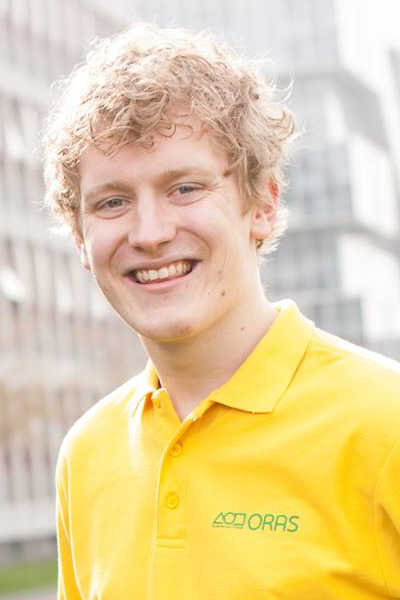
\includegraphics[scale=0.2]{mathijs.png} &

\includegraphics[scale=0.2]{jasper.png}  \\
Ruben Bes	& Mathijs Hoogland	& Jasper Denkers\\
rbes 		& mhhoogland 		& jdenkers\\
4227492 	& 4237676 			& 4212584\\
\end{tabular}
\end{table}

\begin{table}[ht]
\centering
\begin{tabular}{cc}
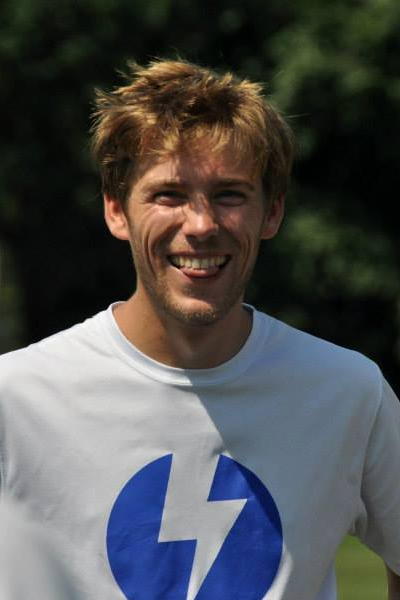
\includegraphics[scale=0.2]{robbert.png} &
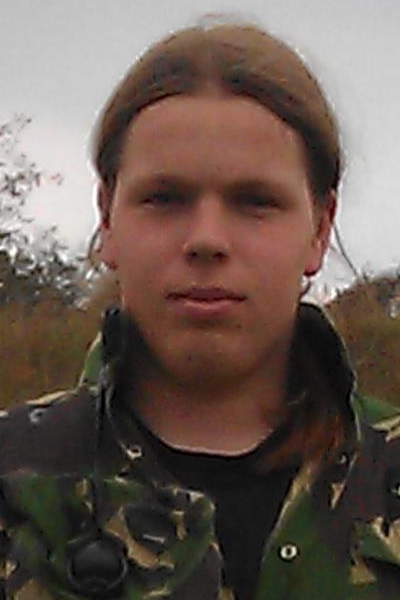
\includegraphics[scale=0.2]{willem.png}  \\
Robbert van Staveren	& Willem Jan Glerum\\
rhvanstaveren 			& wglerum\\
1527118					& 4141040\\
\end{tabular}
\end{table}

\vfill
{\large \today}
\end{center}

\end{titlepage}

\begin{landscape}
\setlength\extrarowheight{5pt}
\begin{longtable}{p{3cm}|p{5cm}|l|l|l|l|p{7cm}}

\textbf{Story} & \textbf{Task} & \textbf{Effort} & \textbf{Assignment} & \textbf{Actual effort} & \textbf{Done} & \textbf{Notes}\\
\hline \hline

A user wants to have an overview of mutations per patient 
& Look for homozygoot mutations & 4 & Mathijs & 10 hours & No & Almost done, had some help from Ruben, was hard to optimize queries to make the processing quick enough.\\
& Look up the exact definition of CADD score and look if the score of 0 can be avoided & 4 & Ruben & 2 hours & Yes & After some help of TA's, it all became clear.\\
& Implement the XY/XX chromosome & 10 & - & - & No & Haven't started yet.\\
\hline

A user wants to view links between genes and proteins related to a mutation 
& Protein visualization per node in the mutation view & 4 & Jasper & 2 & Yes & It was a challenge to design the queries that gave the proper data.\\
& Link diseases to genes & 4 & Ruben & 3 hours & Yes & Had to make a few getters and setters and perform shotgun surgery\\
& Show multiple mutations per graph & 6 & Jasper \& Robbert & 3 hours & No & Haven't had enough time to finish it.\\
& Extend the proteine graph (Make them clickable) & 3 & Robbert \& Jasper & 4 hours & Yes & Wasn't too difficult.\\
& And make them click-able & 1 & Jasper & 1 hour & Yes & After Robbert finished the extending, making them click-able was quite simple.\\
\hline

A user looks at an overview of the location of a mutation & Link Ensemble ID to String database & 4 & Willem Jan & 4 hours & Yes. & Was not very hard once I found out how they had to be linked.\\
& Store GTF information in database & 4 & Willem Jan & 6 hours & Yes & Was hard to store the GTF information in the database, figured it out after some trial and error.\\
& Look if other genes are near the starting point of a mutation & 6 & Willem Jan & 3 hours & No & Have found 1, but want to have more.\\
& Show neighbouring mutations & 6 & - & - & No & Haven't started yet.\\
\hline

Database testing 
& Test database, mocking doesn't work, use a test database & 8 & Willem Jan & 6 hours & Yes & Had to implement the service-interface pattern.\\
& Give proper errors when database fails & 4 & - & - & No & Haven't started yet.\\
\hline

A user logs in and views basic information 
& Optimize dashboard information & 2 & - & - & No & Haven't started yet.\\
& Make breadcrumbs on each page & 2 & Jasper & 2 hours & Yes & Wasn't that hard to implement.\\
\hline

Deliverables 
& Scrum plan 4 week 7 & 1 & Willem Jan & 1 hour & Yes & None.\\
& Scrum reflection 4 week 7 & 2 & Mathijs & 1 hour & Yes & None.\\
\hline
\end{longtable}
\end{landscape}

\section*{General Reflection}
When we look at our scrum reflection, the first thing that we see is that there were quite a couple of tasks that we weren't able to start with. This was mainly because most tasks took more time then we expected, we lost (or invested?) a lot of time in making proper queries and looking through database schemas. We would also like to point out that we have not thought clearly about the second day of 'Pinksteren'.\\
There were also quite a lot of bugs that we had to find and repair, to give an example: in our original implementation, the child's alleles weren't able to be compared with the alleles of the parents. This was because of a bug in the implementation of the mutation class, what was fixed after some research. \\
Another thing quite some time was spent on, is getting certain things clarified. There are a number of things unknown to us, mostly because it is part of the context and we therefore do not know about. It usually consumed time of one or two members of the team, because they are discussing what it really means, and some time to write an email and receive an answer from the TAs.
\end{document}